\documentclass[11pt]{article}
\usepackage[T1]{fontenc}
\usepackage[utf8]{inputenc}
\usepackage{amsmath,amssymb,amsthm,mathtools}
\usepackage{lmodern}
\usepackage[margin=1.05in]{geometry}
\usepackage{microtype,booktabs,tikz}
\usetikzlibrary{arrows.meta}
\usepackage[colorlinks=true,allcolors=blue]{hyperref}
\newcommand{\C}{\mathbb C}
\newcommand{\T}{\mathbb T}
\newcommand{\D}{\mathbb D}
\newcommand{\HS}[1]{\lvert #1\rvert_2}
\DeclareMathOperator{\tr}{tr}
\DeclareMathOperator{\Rea}{Re}
\DeclareMathOperator{\diag}{diag}
\DeclareMathOperator{\dist}{dist}
\newtheorem{theorem}{Theorem}[section]
\newtheorem{lemma}[theorem]{Lemma}
\newtheorem{proposition}[theorem]{Proposition}
\theoremstyle{remark}\newtheorem{remark}[theorem]{Remark}
\numberwithin{equation}{section}
\setlength{\emergencystretch}{2em}
\hypersetup{pdftitle={A direct proof of the complete Crouzeix inequality},pdfauthor={OpenAI}}
\pdftrailerid{}
\title{A direct proof of the complete Crouzeix inequality}
\author{OpenAI}
\date{September 26, 2026}
\begin{document}
\maketitle
\begin{abstract}
We give a direct proof of the sharp constant-two numerical-range inequality
for matrix-valued polynomials in all finite base and coefficient dimensions.
This resolves the complete Crouzeix conjecture in its matrix formulation,
including matrices whose numerical ranges are points or line segments.
\end{abstract}
\section{Introduction}\label{sec:intro}
The numerical range of a matrix $A\in M_n(\C)$ is
\[
 W(A)=\{u^*Au:u\in\C^n,\ u^*u=1\}.
\]
It is a compact convex set containing the spectrum. For a normal matrix,
the spectral theorem controls polynomial evaluation by values on the
spectrum. For a nonnormal matrix, the spectrum alone cannot provide the
same control: even a nonzero nilpotent matrix has spectrum $\{0\}$.
The numerical range retains enough information to give a universal bound.

We allow matrix coefficients. If
$P(z)=\sum_{k=0}^d B_kz^k$ with $B_k\in M_m(\C)$, set
\[
 P[A]=\sum_{k=0}^d A^k\otimes B_k.
\]
The base space $\C^n$ is the first tensor factor. All operator norms
come from the Euclidean inner products and their Hilbert tensor products.
The complete Crouzeix conjecture asks whether the constant two holds
uniformly in the coefficient dimension $m$, the base dimension, and the degree.

\begin{theorem}\label{thm:main}
For every pair of positive integers $n,m$, every $A\in M_n(\C)$,
every nonnegative integer $d$, and every polynomial
$P(z)=\sum_{k=0}^d B_kz^k$ with $B_k\in M_m(\C)$,
\begin{equation}\label{eq:main}
 \|P[A]\|\le2\max_{z\in W(A)}\|P(z)\|.
\end{equation}
The constant two cannot be decreased uniformly over $n,m$, and $d$.
\end{theorem}

The estimate includes point and segment numerical ranges. Its complete
character is the uniformity in $m$: a scalar proof need not survive
matrix amplification, because coefficient matrices need not commute.
The argument below keeps their multiplication order, using the two
products $FG$ and $GF$ separately.

\subsection*{Earlier bounds and related arguments}
Crouzeix formulated the scalar constant-two question in 2004 and proved a
universal complete bound of $11.08$ in 2007
\cite{Crouzeix2004,Crouzeix2007}.
Positive boundary representations developed by Delyon and Delyon
\cite{DelyonDelyon1999} supply an important part of the numerical-range
method. Crouzeix and Palencia combined a positive double-layer potential
with the Cauchy transform of conjugate boundary data to obtain the
complete bound $1+\sqrt2$ \cite{CrouzeixPalencia2017}; Ransford and
Schwenninger simplified its final norm argument
\cite{RansfordSchwenninger2018}.
For all base matrices of order two, Badea, Crouzeix, and Delyon obtained
the complete constant two. In the nonnormal case, they make the conformal
image of the matrix a contraction by a similarity with condition number at
most two, using the numerical-range ellipse \cite{BadeaCrouzeixDelyon2006}.

Recent scalar proofs include work of Jin \cite{Jin2026},
Lorist and Schwenninger \cite{LoristSchwenninger2026}, and Luo
\cite{Luo2026}.
Lorist and Schwenninger's Theorem~3 applies to scalar rational functions
of bounded Hilbert-space operators; their Section~3(iv) explains why the
commutation used in that proof does not automatically persist under
amplification. \AA hag, Czy{\.{z}}, and Virtanen prove the complete
inequality for base matrices of order at most three, with arbitrary
coefficient dimension \cite[Theorem~1.1]{AhagCzyzVirtanen2026}.
The scalar results fix $m=1$, while the latter complete result restricts
the base dimension; Theorem~\ref{thm:main} leaves these dimensions independent.

The use of Faber polynomials in numerical-range functional calculus has
precedents in \cite{Beckermann2005,BeckermannCrouzeix2014}.
Lorist and Schwenninger use a norm-attaining vector in their scalar
argument \cite[Lemma~1]{LoristSchwenninger2026}, while Luo chooses an
explicit top singular pair \cite[Section~3, equations~(21)--(22)]{Luo2026}.
In their complete constant-two proof for weighted shift matrices, Crouzeix
and Greenbaum use a scalar extremal function and a norm-attaining vector
after a similarity reduction
\cite[Section~3, proof of Theorem~2]{CrouzeixGreenbaum2025}.
Here a Faber coefficient estimate controls the two diagonal functionals obtained by placing a test
polynomial on each side of the polynomial being estimated.

A separate structural proof of the complete inequality is given in
\cite{OpenAI2026Complete}. For a bounded convex domain $\Omega$ with
regular real-analytic boundary and $W(A)\subset\Omega$, it constructs a
positive definite $S$ with $\|S\|\|S^{-1}\|\le2$ such that
$S f(A)S^{-1}$ is a contraction, where $f:\Omega\to\D$ is an interior
conformal map and $\D=\{z\in\C:|z|<1\}$. The same $S$, obtained from a
minimizing metric, gives one continuous normalized positive boundary density representing
the calculus of $SAS^{-1}$ for every coefficient dimension and every
matrix function holomorphic near $\overline\Omega$
\cite[Theorems~1.2--1.3 and Proposition~2.1]{OpenAI2026Complete}.
The direct proof below estimates one polynomial at a time. Its exterior
kernel, marginal identities, and positive block comparison have counterparts
in \cite[Propositions~3.1 and~3.3 and Lemma~5.1]{OpenAI2026Complete};
Sections~\ref{sec:coefficients}--\ref{sec:matrix} prove the specific
coefficient, resolvent, and block estimates used here.

\subsection*{How the coefficients give the sharp bound}
First place $W(A)$ strictly inside an analytic convex domain $\Omega$.
An exterior conformal map $h$ parametrizes its boundary by the unit circle.
Expanding the Cauchy kernel at infinity defines scalar polynomials $b_k$ of degree
$k$. For $k\ge1$, the boundary value $b_k\circ h$ has the positive Fourier
term $\lambda^k$ and an otherwise strictly negative expansion. In
Section~\ref{sec:coefficients}, a nonnegative kernel with integral one in
each variable makes the map from the positive part to the negative part an
$L^2$ contraction. Thus, for $G=\sum_k b_kC_k$, its squared boundary
Hilbert--Schmidt norm lies between the square sum of its coefficient norms
and that sum with weight two on every nonconstant coefficient.

For a polynomial $F$ normalized by its boundary operator norm, choose a
unit top singular pair $x,y$ for $F[A]$. The resolvent
$R(\lambda)=\lambda h'(\lambda)(h(\lambda)I-A)^{-1}$ supplies the
coefficient arrays representing the three functionals
$y^*G[A]x$, $x^*G[A]x$, and $y^*G[A]y$. The first is bounded by a
coefficient Hilbert norm. Testing it on $FG$ and $GF$ separately gives
bounds for the other two. Their squared dual coefficient norms have reciprocal
weights: one on the constant coefficient and one half on the others.
These are exactly the weights in the squared Fourier norms of the corresponding
Hermitian diagonal compressions, after a common factor of four.

Section~\ref{sec:matrix} completes the comparison. The numerical-range
condition makes $R+R^*$ positive, so its compression to a two-by-two
block bounds the off-diagonal boundary norm by the two diagonal norms.
The cross term retains all coefficients of the first functional, including
its constant coefficient. The resulting inequality gives the sharp bound
two. Section~\ref{sec:limit} then shrinks analytic convex neighborhoods
to an arbitrary numerical range and proves sharpness with a two-by-two
nilpotent matrix. Appendix~\ref{sec:collar} supplies the exterior collar
using classical conformal mapping and reflection theorems.
\section{Exterior coordinates and coefficient estimates}\label{sec:coefficients}
In this section $\Omega$ is a bounded open convex set with regular real-analytic Jordan boundary. We work with a supplied exterior conformal map $h$ that is one-to-one on $|\lambda|>r$, including infinity on the Riemann sphere, for some $0<r<1$. It maps $|\lambda|>1$ onto $\C\setminus\overline\Omega$ and has a simple pole at infinity, with expansion
\begin{equation}\label{eq:h}
 h(\lambda)=c\lambda+c_0+O(\lambda^{-1}),\qquad c\ne0.
\end{equation}
Appendix~\ref{sec:collar} supplies such a coordinate for every domain under consideration. Here we use it to compare polynomial coefficients with boundary norms.

The map $h$ sends $\T=\{\lambda:|\lambda|=1\}$ onto $\partial\Omega$. Put $q(\lambda)=\lambda h'(\lambda)$. On $\T$, the vector $q(\lambda)$ is an outward normal and $iq(\lambda)$ is a positively oriented tangent. Hence
\begin{equation}\label{eq:support}
 \Re\bigl(\overline{q(\lambda)}(h(\lambda)-z)\bigr)\ge0
 \quad(\lambda\in\T,\ z\in\overline\Omega).
\end{equation}
Figure~\ref{fig:normal} illustrates this supporting-line relation.

\begin{figure}[ht]
\centering
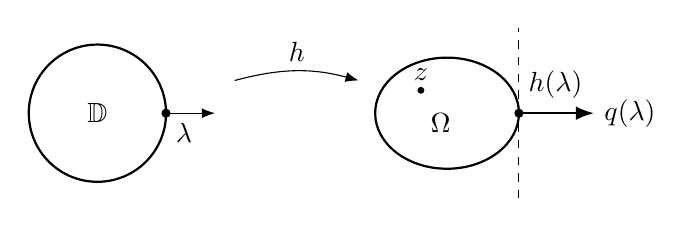
\begin{tikzpicture}[scale=.83,>=Latex]
 \draw[thick] (0,0) circle (1.05);
 \node at (0,0) {$\D$};
 \fill (1.05,0) circle (2pt);
 \node[below right] at (1.05,0) {$\lambda$};
 \draw[->] (1.05,0) -- (1.8,0);
 \draw[->] (2.1,.5) to[bend left=15] node[above] {$h$} (4,.5);
 \draw[thick] (5.35,0) ellipse (1.1 and .85);
 \node at (5.25,-.15) {$\Omega$};
 \draw[dashed] (6.45,-1.3) -- (6.45,1.3);
 \fill (6.45,0) circle (2pt);
 \draw[->,thick] (6.45,0) -- (7.6,0) node[right] {$q(\lambda)$};
 \node[above right] at (6.45,.08) {$h(\lambda)$};
 \fill (4.95,.35) circle (1.5pt);
 \node[above] at (4.95,.35) {$z$};
\end{tikzpicture}
\caption{The map $h$ sends the exterior of the circle to the exterior of the domain; the supporting line is shown schematically. Increasing the circle radius gives the outward normal $q(\lambda)$; convexity places every $z\in\overline\Omega$ on the inner side of the line.}
\label{fig:normal}
\end{figure}


Every circle integral below uses $d\tau(e^{it})=dt/(2\pi)$.

We use the unnormalized Hilbert--Schmidt norm $\HS C=(\tr(C^*C))^{1/2}$, which makes each finite-dimensional matrix space a Hilbert space.

\begin{theorem}[Exterior Faber coefficients and the positive kernel]\label{lem:faber}
Let $\Omega$ be a bounded convex domain with regular real-analytic Jordan boundary. Let $h$ be meromorphic and one-to-one on $|\lambda|>r$ including infinity, where $0<r<1$, with a simple pole at infinity as in \eqref{eq:h}, and mapping $|\lambda|>1$ onto $\C\setminus\overline\Omega$. Put $q(\lambda)=\lambda h'(\lambda)$ and define $b_k(z)$ by expansion at infinity:
\begin{equation}\label{eq:faber}
 \frac{q(\lambda)}{h(\lambda)-z}=\sum_{k\ge0}b_k(z)\lambda^{-k}.
\end{equation}
Then $b_0=1$, and each $b_k$ is a polynomial of degree $k$ with leading coefficient $c^{-k}$. There are scalars $s_{kj}$, $k,j\ge1$, such that
\begin{equation}\label{eq:boundary-basis}
 b_k(h(\mu))=\mu^k+\sum_{j\ge1}s_{kj}\mu^{-j}\quad(k\ge1).
\end{equation}
The function
\begin{equation}\label{eq:s}
 s(\lambda,\mu)=\frac{q(\lambda)}{h(\lambda)-h(\mu)}-\frac{\lambda}{\lambda-\mu}
 =\sum_{k,j\ge1}s_{kj}\lambda^{-k}\mu^{-j}
\end{equation}
extends holomorphically across the diagonal and both infinities in $|\lambda|,|\mu|>r$. For every $r<\rho<1$ there is a constant $C_\rho$ with
$|s_{kj}|\le C_\rho\rho^{k+j}$. The series converges normally on
the exterior product collar: it converges absolutely and uniformly on
every compact subset, including subsets meeting either infinity.
In particular it converges absolutely and uniformly on $\T^2$. The continuous kernel
\[
 K(\lambda,\mu)=1+s(\lambda,\mu)+\overline{s(\lambda,\mu)}
\]
is nonnegative and has integral one in each variable with the other fixed.
\end{theorem}

\begin{proof}
Expanding the denominator in \eqref{eq:faber} after factoring $c\lambda$ shows that its $k$th coefficient is a polynomial of degree $k$ with leading term $c^{-k}z^k$. The constant coefficient is one. In particular, the $b_k$ form a basis of the scalar polynomials.

For the joint extension, consider
\[
 H(\lambda,\mu)=\frac{h(\lambda)-h(\mu)}{\lambda-\mu}.
\]
Write $u=\lambda^{-1}$, $v=\mu^{-1}$ and $h(\lambda)=c\lambda+g(u)$, where $g$ is holomorphic on $|u|<r^{-1}$. Then
\begin{equation}\label{eq:H}
 H=c-uv\frac{g(u)-g(v)}{u-v}.
\end{equation}
The divided difference of $g$ is jointly holomorphic, with diagonal value $g'(u)$, so this formula also covers either or both infinities. Off the diagonal and away from the axes, $H$ is nonzero by injectivity of $h$. On the diagonal it equals $h'(\lambda)\ne0$; on either axis it equals $c$. Thus it has no zeros on the reciprocal bidisk.

Direct differentiation gives $s=\lambda\partial_\lambda H/H=-u\partial_uH/H$. This function is holomorphic and vanishes on both reciprocal axes. Its Taylor series has precisely the strictly mixed powers in \eqref{eq:s}. For any $r<\rho<1$, Cauchy estimates on the closed reciprocal bidisk
of radius $\rho^{-1}$ give a constant $C_\rho$ with
$|s_{kj}|\le C_\rho\rho^{k+j}$. On a compact subset of the exterior
product collar, choose $\sigma>r$ below all finite coordinate moduli,
and then $r<\rho<\min(1,\sigma)$. The resulting geometric double
series dominates the Laurent series uniformly there; terms vanish on
the reciprocal axes. This proves normal convergence throughout the
product collar and absolute uniform convergence on the boundary. Comparing coefficients at $\lambda=\infty$ in \eqref{eq:s}, first for fixed finite $\mu$ in the exterior collar, yields \eqref{eq:boundary-basis}.

For distinct $\lambda,\mu\in\T$, one has $2\Re(\lambda/(\lambda-\mu))=1$, and therefore
\[
 K(\lambda,\mu)=2\Re\frac{q(\lambda)}{h(\lambda)-h(\mu)}\ge0
\]
by \eqref{eq:support}. Continuity gives the same sign on the diagonal. Every term of $s$ and of its conjugate has nonzero frequency in each variable. Their integrals in either variable vanish, proving both normalizations.
\end{proof}

To identify the basis, let $\Phi=h^{-1}$ in the exterior. Equation~\eqref{eq:boundary-basis}, which holds throughout the exterior collar, gives $b_k(z)-\Phi(z)^k=O(z^{-1})$ at infinity. Thus $b_k$ is the polynomial part of $\Phi^k$, the Faber polynomial associated with the chosen exterior coordinate. The usual normalization chooses the phase of $h$ so that $c>0$ \cite{Beckermann2005,BeckermannCrouzeix2014}.

These mixed coefficients are differentiated Grunsky coefficients.
The classical normalization gives a weighted coefficient inequality
\cite[equations~(1.1)--(1.3)]{BeckermannStylianopoulos2018};
the unweighted estimate used here follows from convexity and the two
angular marginal identities.

The two normalizations in Theorem~\ref{lem:faber} use the same exterior circle measure. Together they control the negative Fourier part of a boundary polynomial by its positive part, as follows.

\begin{proposition}[The coefficient norm estimate]\label{prop:coefficients}
For every positive integer $m$ and every $M_m(\C)$-valued polynomial $G(z)=\sum_{k=0}^N b_k(z)C_k$,
\begin{equation}\label{eq:coefficient-estimate}
 \sum_{k=0}^N\HS{C_k}^2
 \le\int_\T\HS{G(h(\mu))}^2\,d\tau(\mu)
 \le\HS{C_0}^2+2\sum_{k=1}^N\HS{C_k}^2.
\end{equation}
\end{proposition}
\begin{proof}
For $u\in L^2(\T;\mathcal H)$ with values in a Hilbert space $\mathcal H$, define
\[
 (Tu)(\mu)=\int_\T K(\lambda,\mu)u(\lambda)\,d\tau(\lambda).
\]
Positivity and the normalization in $\lambda$ imply
$\|(Tu)(\mu)\|^2\le\int K(\lambda,\mu)\|u(\lambda)\|^2d\tau(\lambda)$.
Integrating in $\mu$ and using the normalization in that variable shows that $T$ is an $L^2$ contraction.

For $u(\lambda)=\sum_{k=1}^N C_k\lambda^k$, only the $s$ term contributes to the integral, so
\begin{equation}\label{eq:kernel-fourier-action}
 (Tu)(\mu)=\sum_{j\ge1}\left(\sum_{k=1}^Ns_{kj}C_k\right)\mu^{-j}.
\end{equation}
All interchanges are justified by the absolute uniform convergence in Theorem~\ref{lem:faber}. In particular,
\[
 \sum_{j\ge1}\HS{\sum_{k=1}^Ns_{kj}C_k}^2\le\sum_{k=1}^N\HS{C_k}^2.
\]
By \eqref{eq:boundary-basis}, the boundary value of $G$ is the sum of its constant term $C_0$, its positive part $u$, and its negative part $Tu$. These have disjoint Fourier supports. Parseval's identity gives
\[
 \int_\T\HS{G\circ h}^2d\tau
 =\HS{C_0}^2+\sum_{k=1}^N\HS{C_k}^2+
   \sum_{j\ge1}\HS{\sum_{k=1}^Ns_{kj}C_k}^2,
\]
which proves both inequalities.
\end{proof}
For comparison with \cite[Proposition~3.1]{OpenAI2026Complete}, the
companion's exterior map $G$ and variables $t,w$ correspond to
$h,\lambda,\mu$, respectively.
The mixed correction is $s(\lambda,\mu)=B(\mu,\lambda)$, so
$s_{kj}=\beta_{jk}$ in that paper's notation. In particular,
\eqref{eq:kernel-fourier-action} uses this coefficient orientation and
does not require symmetry of the kernel.
\section{Singular vectors and the amplified estimate}\label{sec:matrix}
Fix $A\in M_n(\C)$ with $W(A)\subset\Omega$.
To estimate the norm of one polynomial evaluation, we form coefficient
functionals from its left and right singular vectors. The resolvent supplies
their coefficient arrays, while its positive Hermitian part compares the
resulting boundary norms. This Hermitian field is the numerical-range double-layer kernel of
\cite{DelyonDelyon1999,CrouzeixPalencia2017}; we prove the required
positivity for the original matrix $A$.

\begin{theorem}[The resolvent expansion and double-layer positivity]\label{lem:resolvent}
Let $\Omega,h,q$, and $(b_k)$ satisfy the hypotheses and conclusions of Theorem~\ref{lem:faber}. For any positive integer $n$ and $A\in M_n(\C)$ with $W(A)\subset\Omega$, on $\T$ let
\begin{equation}\label{eq:R}
 R(\lambda)=q(\lambda)(h(\lambda)I-A)^{-1}.
\end{equation}
Then
\[
 R(\lambda)=\sum_{k\ge0}b_k(A)\lambda^{-k},\qquad R(\lambda)+R(\lambda)^*\succeq0.
\]
For the fixed $A,h$, there are constants $C<\infty$ and $0<\theta<1$
such that $\|b_k(A)\|\le C\theta^k$ for all $k\ge0$. Thus the series
converges absolutely and uniformly on $\T$. In particular,
$\int_\T R\,d\tau=I$ and $\int_\T(R+R^*)\,d\tau=2I$.
\end{theorem}
\begin{proof}
Every eigenvalue of $A$ belongs to $W(A)$, by testing a unit eigenvector. Thus the exterior resolvent is defined on and outside the boundary. Compactness of the circle and strict spectral separation allow a smaller collar $|\lambda|>r_A$, with $r<r_A<1$, on which it remains holomorphic, including infinity where $R(\infty)=I$. Expansion at infinity gives the coefficients $b_k(A)$: this follows either by the geometric resolvent series for large $|h(\lambda)|$ or by substituting $A$ into the polynomial coefficient identities in \eqref{eq:faber}. Choose $r_A<\theta<1$. Cauchy estimates on the reciprocal circle of
radius $\theta^{-1}$ give the stated geometric bound. They imply
absolute uniform convergence on $\T$, and its constant coefficient
$b_0(A)=I$ gives both integrals.

For $B=h(\lambda)I-A$, direct congruence gives
\[
 B^*(R+R^*)B=\overline{q(\lambda)}B+q(\lambda)B^*.
\]
For each unit vector $v$, the quadratic form on the right is
$2\Re(\overline{q(\lambda)}(h(\lambda)-v^*Av))$, which is nonnegative by \eqref{eq:support}. Invertibility of $B$ proves positivity.
\end{proof}

\begin{theorem}[The bound on an analytic convex domain]\label{thm:domain}
For positive integers $n,m$, let $\Omega\subset\C$ be bounded, open, and convex with regular real-analytic Jordan boundary, and let $A\in M_n(\C)$ satisfy $W(A)\subset\Omega$. For every $M_m(\C)$-valued polynomial $F$ with $\|F(z)\|\le1$ on $\partial\Omega$, one has $\|F[A]\|\le2$.
\end{theorem}
\begin{proof}
Choose $h$ from Lemma~\ref{lem:exterior-collar} and apply
Theorem~\ref{lem:faber} to this coordinate.
Put $\gamma=\|F[A]\|$. There is nothing to prove if $\gamma=0$. Otherwise choose unit singular vectors $x,y\in\C^n\otimes\C^m$ such that
\begin{equation}\label{eq:singular}
 F[A]x=\gamma y,\qquad F[A]^*y=\gamma x.
\end{equation}
Write $x=\sum_{i=1}^mXe_i\otimes e_i$ and $y=\sum_{i=1}^mYe_i\otimes e_i$, where $X,Y$ are $n$-by-$m$ matrices and $(e_i)$ is the standard basis of $\C^m$. For the resolvent in Theorem~\ref{lem:resolvent}, define matrix functions
\[
 P=X^*RX,\quad Q=Y^*RY,\quad M=Y^*RX,\quad L=X^*RY.
\]
Subscripts $k\ge0$ denote the coefficients of $\lambda^{-k}$, so $M_k=Y^*b_k(A)X$, for example. By Theorem~\ref{lem:resolvent}, all four series converge absolutely and uniformly on $\T$, and their coefficient sequences are square summable. Since $b_0=1$,
\begin{equation}\label{eq:means}
 P_0=X^*X=P_0^*,\qquad Q_0=Y^*Y=Q_0^*,\qquad L_0^*=M_0.
\end{equation}
Set $a^2=\sum_{k\ge0}\HS{M_k}^2$. We will bound the squared
boundary $L^2$ Hilbert--Schmidt norms of $P+P^*$ and $Q+Q^*$
above by $4a^2/\gamma^2$ each, and that of $M+L^*$ below by $a^2$.
Positivity will then compare these quantities and force $\gamma\le2$.

\emph{The off-diagonal coefficient functional.}
For a polynomial $G=\sum_k b_kC_k$, direct expansion in the tensor basis gives
\begin{equation}\label{eq:pairing}
 y^*G[A]x=\sum_{k,i,j}(M_k)_{ij}(C_k)_{ij}.
\end{equation}
Indeed, $C_ke_j=\sum_i(C_k)_{ij}e_i$ in the coefficient factor, leaving $(Ye_i)^*b_k(A)Xe_j$ in the base factor. Equation~\eqref{eq:pairing} is the bilinear entry pairing of the two coefficient arrays. Cauchy--Schwarz gives
\begin{equation}\label{eq:crossfunctional}
 |y^*G[A]x|\le a\left(\sum_k\HS{C_k}^2\right)^{1/2}.
\end{equation}
Taking $G=F$ and using \eqref{eq:singular} shows that $a>0$.

\emph{The two ordered tests.}
Polynomial evaluation respects multiplication in its given order. Explicitly, if $F(z)=\sum_iD_iz^i$ and $G(z)=\sum_jE_jz^j$, then
\[
 (FG)[A]=\sum_{i,j}A^{i+j}\otimes D_iE_j=F[A]G[A],
\]
and the reversed product has coefficients $E_jD_i$. Hence
\begin{equation}\label{eq:ordered-products}
 y^*(FG)[A]x=\gamma x^*G[A]x,\qquad
 y^*(GF)[A]x=\gamma y^*G[A]y.
\end{equation}
Write the full finite Faber expansions as
\[
 FG=\sum_k b_kU_k,\qquad GF=\sum_k b_kV_k,
 \qquad \|H\|_\partial^2=\int_\T\HS{H(h(\mu))}^2\,d\tau(\mu).
\]
The functional in \eqref{eq:crossfunctional} uses all $M_k$, so it applies
to these full expansions for every finite degree. Apply it to the two
identities in \eqref{eq:ordered-products}. The lower coefficient estimate
in Proposition~\ref{prop:coefficients} and the two boundary multiplier
bounds give
\begin{align*}
 \gamma|x^*G[A]x|
 &\le a\Bigl(\sum_k\HS{U_k}^2\Bigr)^{1/2}
 \le a\|FG\|_\partial\le a\|G\|_\partial,\\
 \gamma|y^*G[A]y|
 &\le a\Bigl(\sum_k\HS{V_k}^2\Bigr)^{1/2}
 \le a\|GF\|_\partial\le a\|G\|_\partial.
\end{align*}
Here $\HS{F(z)G(z)}\le\|F(z)\|\HS{G(z)}$ and
$\HS{G(z)F(z)}\le\HS{G(z)}\|F(z)\|$ are used in their
respective orders. The upper coefficient estimate for $G$ now gives
\begin{equation}\label{eq:diagonal-functional}
 \max\{|x^*G[A]x|,|y^*G[A]y|\}
 \le\frac a\gamma
 \left(\HS{C_0}^2+2\sum_{k\ge1}\HS{C_k}^2\right)^{1/2}.
\end{equation}
The entries paired with $C_k$ in these two functionals are respectively those of $P_k$ and $Q_k$, by the calculation in \eqref{eq:pairing}. The weighted coefficient norm on the right gives reciprocal weights on these two coefficient sequences:
\begin{equation}\label{eq:weighted-dual}
 \HS{P_0}^2+\tfrac12\sum_{k\ge1}\HS{P_k}^2\le a^2/\gamma^2,
 \qquad
 \HS{Q_0}^2+\tfrac12\sum_{k\ge1}\HS{Q_k}^2\le a^2/\gamma^2.
\end{equation}
For the first inequality, set
$d_N=\HS{P_0}^2+\tfrac12\sum_{k=1}^N\HS{P_k}^2$
and test \eqref{eq:diagonal-functional} with $C_0=\overline{P_0}$,
$C_k=\overline{P_k}/2$ for $1\le k\le N$, and $C_k=0$ otherwise;
bars mean entrywise conjugation. The paired value is $d_N$, and the squared
weighted test norm is also $d_N$. Hence
$d_N\le(a/\gamma)\sqrt{d_N}$, which gives $d_N\le a^2/\gamma^2$
including when $d_N=0$. Letting $N\to\infty$ proves the first bound.
The same finite tests with $Q_k$ prove the second.

\emph{The boundary norms of the three blocks.}
The compression of $R+R^*$ by $[X\ Y]$ has diagonal blocks $P+P^*$,
$Q+Q^*$ and lower off-diagonal block $M+L^*$. We first compute their
boundary norms. In the diagonal fields, \eqref{eq:means} makes the
constant term twice $P_0$ or $Q_0$. For $k\ge1$, the coefficients $P_k$
and $P_k^*$ occur at frequencies $-k$ and $k$ and have equal
Hilbert--Schmidt norms; the same holds for $Q_k$ and $Q_k^*$.
Parseval therefore gives four times the reciprocal weighted sum in
\eqref{eq:weighted-dual}:
\begin{equation}\label{eq:diagonal-L2}
 \int_\T\HS{P+P^*}^2d\tau
 =4\left(\HS{P_0}^2+\tfrac12\sum_{k\ge1}\HS{P_k}^2\right)
 \le4a^2/\gamma^2,
\end{equation}
and the same identity and bound hold for $Q+Q^*$.

For the cross field, $L_0^*=M_0$ makes the constant term $2M_0$.
Its negative coefficients are $M_k$ for $k\ge1$ and its positive
coefficients are $L_k^*$ for $k\ge1$. Consequently
\begin{equation}\label{eq:cross-L2}
 \int_\T\HS{M+L^*}^2d\tau
 =4\HS{M_0}^2+\sum_{k\ge1}\bigl(\HS{M_k}^2+\HS{L_k}^2\bigr)
 \ge a^2.
\end{equation}

\emph{The positive block comparison.}
Theorem~\ref{lem:resolvent} gives $R+R^*\succeq0$. Its compression by the
$n$-by-$2m$ matrix $[X\ Y]$ is therefore
\[
 \Delta=\begin{pmatrix}P+P^*&L+M^*\\M+L^*&Q+Q^*\end{pmatrix}\succeq0.
\]
For $J=\diag(I_m,-I_m)$, the matrix $J\Delta J$ is also positive, so
\[
 0\le\tr\bigl(\Delta^{1/2}(J\Delta J)\Delta^{1/2}\bigr)
 =\tr(\Delta J\Delta J)
 =\HS{P+P^*}^2+\HS{Q+Q^*}^2-2\HS{M+L^*}^2.
\]
Integrating this inequality and using \eqref{eq:diagonal-L2} and \eqref{eq:cross-L2} yields
\[
 2a^2\le2\int_\T\HS{M+L^*}^2d\tau
 \le\int_\T\bigl(\HS{P+P^*}^2+\HS{Q+Q^*}^2\bigr)d\tau
 \le8a^2/\gamma^2.
\]
Since $a>0$, this proves $\gamma\le2$.
\end{proof}
\section{Enclosing domains and arbitrary numerical ranges}\label{sec:limit}
Theorem~\ref{thm:domain} applies on an analytic convex neighborhood. We now construct such neighborhoods even for compact convex sets with empty interior, and then shrink them to $W(A)$.

\begin{lemma}[Analytic convex outer approximation]\label{lem:approx}
Let $K\subset\C$ be nonempty, compact, and convex. There are bounded convex open domains $\Omega_j$ with regular real-analytic Jordan boundaries such that $K\subset\Omega_j$ and
\[
 \sup_{z\in\overline\Omega_j}\dist(z,K)\longrightarrow0.
\]
\end{lemma}
\begin{proof}
For $0<\delta<1$, choose a finite Euclidean $\delta$-net $D_\delta$ of unit directions that includes $1,-1,i,-i$. Let $s_K(\nu)=\max_{z\in K}\Re(\bar\nu z)$ be the support function. Choose $t_\delta>0$ with $|D_\delta|e^{-t_\delta\delta}<1$, and define
\[
 \Phi_\delta(z)=\sum_{\nu\in D_\delta}
 \exp\bigl(t_\delta(\Re(\bar\nu z)-s_K(\nu)-\delta)\bigr),
 \qquad \Omega_\delta=\{z:\Phi_\delta(z)<1\}.
\]
Each point of $K$ satisfies $\Phi_\delta<1$, so $K\subset\Omega_\delta$.
If $\Phi_\delta(z)\le1$, each positive summand is at most one, and hence
\[
 \Re(\bar\nu z)\le s_K(\nu)+\delta\qquad(\nu\in D_\delta).
\]
In particular, the four axis directions give
\[
 \begin{aligned}
 \min_{w\in K}\Re w-\delta&\le\Re z\le\max_{w\in K}\Re w+\delta,\\
 \min_{w\in K}\Im w-\delta&\le\Im z\le\max_{w\in K}\Im w+\delta.
 \end{aligned}
\]
Thus one fixed rectangle contains every closed sublevel for $0<\delta<1$.

The Hessian is a sum of positive multiples of $\nu\nu^{\mathsf T}$ after identifying $\C$ with $\mathbb R^2$. The four axis directions ensure it is positive definite. Thus $\Phi_\delta$ is strictly convex and real analytic.

The gradient cannot vanish at level one: a critical point of a differentiable convex function is a global minimum, whereas every point of $K$ has value less than one. The implicit function theorem therefore makes that level a regular real-analytic curve. The open sublevel set is bounded and convex with nonempty interior. Fix an interior point. Each ray from it crosses level one exactly once; convexity and boundedness give existence and uniqueness. Radial projection from the compact boundary to the circle is a continuous bijection, hence a homeomorphism. The boundary is a Jordan curve, and $\overline\Omega_\delta=\{\Phi_\delta\le1\}$.

It remains to bound the distance of this sublevel from $K$. For
$z\in\overline\Omega_\delta\setminus K$, let $w\in K$ be nearest to $z$,
put $d=|z-w|$ and $\nu=(z-w)/d$, and choose $\mu\in D_\delta$ with
$|\mu-\nu|\le\delta$. Choose $v\in K$ attaining $s_K(\mu)$.
Since $w+t(v-w)\in K$ for $0\le t\le1$, minimality of $w$ gives
$\Re(\bar\nu(v-w))\le0$.
Using this inequality and the support inequality for $\mu$, we obtain
\[
 \begin{aligned}
 (1-\delta)d
 &\le\Re(\bar\mu(z-w))\\
 &\le\Re(\bar\mu(v-w))+\delta\\
 &\le\delta|v-w|+\delta
 \le\delta\bigl(1+\operatorname{diam}K\bigr).
 \end{aligned}
\]
The first and third inequalities use $|\mu-\nu|\le\delta$. Points of $K$
have distance zero, so
\[
 \sup_{z\in\overline\Omega_\delta}\dist(z,K)
 \le\frac{\delta(1+\operatorname{diam}K)}{1-\delta}\longrightarrow0.
\]
Taking, for example, $\delta_j=1/(j+1)$ completes the construction.
\end{proof}

\begin{proof}[Proof of Theorem~\ref{thm:main}]
Compactness of $W(A)$ follows from compactness of the unit sphere. We recall a short proof of the Toeplitz--Hausdorff convexity theorem \cite{Toeplitz1918,Hausdorff1919}. To join two numerical-range values, compress $A$ to the span of their unit testing vectors. If that span has dimension one there is nothing to prove. In dimension two, its quadratic form on unit vectors $(u,v)$ is a complex-valued real-affine function of
\[
 (2\Re(\bar uv),\ 2\Im(\bar uv),\ |u|^2-|v|^2),
\]
which ranges over the full unit sphere in $\mathbb R^3$. The linear part of a map from $\mathbb R^3$ to $\mathbb R^2$ has a nonzero kernel. Any point of the unit ball can be moved in a kernel direction to the sphere without changing its image. Thus the images of the sphere and ball coincide, and this image is convex. Its segment between the chosen values belongs to the numerical range of the compression and hence to $W(A)$.

Apply Lemma~\ref{lem:approx} with $K=W(A)$. By scaling Theorem~\ref{thm:domain},
\[
 \|P[A]\|\le2\max_{z\in\overline\Omega_j}\|P(z)\|.
\]
If this maximum is zero, each entry of $P$ vanishes on an open set and the polynomial is identically zero, making the inequality immediate. Otherwise divide $P$ by the maximum to invoke that theorem. All $\overline\Omega_j$ lie in one compact set. Uniform continuity of the fixed function $z\mapsto\|P(z)\|$, the containment of $K$, and the uniform distance convergence imply convergence of these maxima to $\max_K\|P\|$. This proves \eqref{eq:main} without any interior assumption on $K$.

For sharpness take $n=2$, $m=1$, $P(z)=z$, and
\[
 A=\begin{pmatrix}0&2\\0&0\end{pmatrix}.
\]
Its norm is two, while $|x^*Ax|=2|x_1x_2|\le1$ for every unit $x$, with equality at $x_1=x_2=1/\sqrt2$. Thus the right-hand maximum in \eqref{eq:main} is one. No smaller universal constant is possible.
\end{proof}
\appendix
\section{The exterior conformal collar}\label{sec:collar}
We record the classical conformal inputs and prove the continuation and global injectivity required in Section~\ref{sec:coefficients}.

\begin{lemma}[Exterior coordinate and a univalent collar]
\label{lem:exterior-collar}
Let $\Omega\subset\mathbb C$ be a bounded convex domain whose boundary
is a regular real-analytic Jordan curve. There are $0<r_0<1$ and a map
$h$, meromorphic on $\{\lambda:|\lambda|>r_0\}\cup\{\infty\}$,
which is one-to-one there as a map of the sphere, has a simple pole at
infinity, and maps $|\lambda|>1$ conformally onto
$\mathbb C\setminus\overline\Omega$. It maps the unit circle onto
$\partial\Omega$ and has an expansion
\[
 h(\lambda)=c\lambda+c_0+\sum_{j\ge1}c_j\lambda^{-j},\qquad c\ne0.
\]
For $\lambda$ on the unit circle, $q(\lambda)=\lambda h'(\lambda)$
is a nonzero outward normal vector at $h(\lambda)$. In particular,
\[
 \operatorname{Re}\bigl(\overline{q(\lambda)}(h(\lambda)-z)\bigr)
 \ge0\qquad (z\in\overline\Omega).
\]
\end{lemma}

\begin{proof}
Fix $z_*\in\Omega$ and apply $z\mapsto1/(z-z_*)$, with infinity
mapped to zero, to the spherical exterior
$(\mathbb C\setminus\overline\Omega)\cup\{\infty\}$. Its image $U$ is
a bounded simply connected domain containing zero, with a regular
real-analytic Jordan boundary. Indeed, each ray from $z_*$ meets
$\partial\Omega$ at a unique positive radius; inversion turns the
exterior portions of these rays into a star-shaped domain about zero.
The Riemann mapping theorem \cite[Chapter~6, Section~1.1, Theorem~1]{Ahlfors1979}
supplies a conformal bijection
$g:\mathbb D\to U$ with $g(0)=0$. Carath\'eodory's Jordan-domain theorem
\cite[Chapter~6, Section~1.2]{Ahlfors1979} extends $g$ to a homeomorphism $\overline{\mathbb D}\to\overline U$.

We justify the stronger boundary continuation needed below. A regular
real-analytic boundary arc has a real-analytic parametrization with
nonzero derivative. Its holomorphic continuation and the holomorphic
inverse-function theorem provide a local coordinate in which the arc
is a real interval and the domain is one side of that interval. Choose
such coordinates at $\zeta\in\partial\mathbb D$ and
$p=g(\zeta)\in\partial U$. Continuity of the boundary extension lets us
shrink the source neighborhood so that $g$ maps its intersection with
$\overline{\mathbb D}$ into the target chart.
The composition representing $g$ in these
coordinates is holomorphic on a half disk, continuous on its real
interval, and real-valued there. Schwarz reflection extends it
holomorphically across the interval
\cite[Chapter~4, Section~6.5; Chapter~6, Sections~1.3--1.4]{Ahlfors1979}. Apply the same procedure to
$g^{-1}$. Shrink the neighborhoods so that the reflected maps can be
composed. Their compositions equal the identity on the original domain
side, and hence throughout a smaller neighborhood by the identity theorem.
Thus the continued $g$ has nonzero derivative at each boundary point.

To patch the local continuations, choose around every
$\zeta\in\partial\mathbb D$ a disk $B(\zeta,R_\zeta)$ carrying such a continuation, agreeing
with $g$ on its intersection with $\mathbb D$. Select finitely many of
the third-radius disks $V_i=B(\zeta_i,R_i/3)$ that cover the circle,
and denote the larger disks by $U_i=B(\zeta_i,R_i)$. If
$V_i\cap V_j\ne\varnothing$ and $R_i\ge R_j$, then
$|\zeta_i-\zeta_j|<(R_i+R_j)/3\le2R_i/3<R_i$.
The connected lens $U_i\cap U_j$ therefore contains $\zeta_j$ and
meets $\mathbb D$. The two continuations coincide there by the identity
theorem. They consequently patch with $g$ to a holomorphic map on
$\mathbb D\cup\bigcup_iV_i$, a neighborhood of the closed disk.

The extension is injective on a smaller neighborhood of the closed
disk. Otherwise, distinct colliding pairs arbitrarily close to that
compact set would have subsequential limits in the closed disk.
Continuity and injectivity on the closed disk identify their limits.
Both points of each pair would then eventually lie in one local
inverse neighborhood of that common limit, a contradiction. By compactness,
this injective neighborhood contains the disk $\{w:|w|<R_0\}$ for some $R_0>1$.
Thus $g$ is univalent on that disk. Its sole zero there
is $0$, and that zero is simple. Set
\[
 h(\lambda)=z_*+\frac1{g(1/\lambda)},\qquad r_0=R_0^{-1}.
\]
This gives all mapping and extension assertions, including the simple
pole with coefficient $c=1/g'(0)\ne0$.

Finally, at $\lambda=e^{i\theta}$ the radial and angular derivatives
are $q(\lambda)$ and $iq(\lambda)$, respectively. They are perpendicular
and nonzero. Increasing the radial parameter enters the exterior of
$\overline\Omega$, so $q(\lambda)$ points outward. The supporting
half-plane property of a smooth convex boundary proves the final
inequality.
\end{proof}
\begin{thebibliography}{99}
\raggedright

\bibitem{AhagCzyzVirtanen2026}
P.~\AA hag, R.~Czy{\.{z}}, and J.~Virtanen,
\emph{The complete Crouzeix conjecture in dimension three and the
Clou\^atre--Ostermann--Ransford conjecture},
\href{https://arxiv.org/abs/2608.27346v4}{arXiv:2608.27346v4}, September 21, 2026.

\bibitem{Ahlfors1979}
L.~V. Ahlfors, \emph{Complex Analysis}, third ed., McGraw--Hill, New York, 1979.

\bibitem{BadeaCrouzeixDelyon2006}
C.~Badea, M.~Crouzeix, and B.~Delyon,
Convex domains and $K$-spectral sets,
\emph{Math. Z.} \textbf{252} (2006), 345--365.
\href{https://doi.org/10.1007/s00209-005-0857-y}{doi:10.1007/s00209-005-0857-y}.

\bibitem{Beckermann2005}
B.~Beckermann, Image num{\'e}rique, GMRES et polyn{\^o}mes de Faber,
\emph{C. R. Math.} \textbf{340} (2005), 855--860.
\href{https://doi.org/10.1016/j.crma.2005.04.027}{doi:10.1016/j.crma.2005.04.027}.

\bibitem{BeckermannCrouzeix2014}
B.~Beckermann and M.~Crouzeix,
Faber polynomials of matrices for non-convex sets,
\emph{Jaen J. Approx.} \textbf{6} (2014), 219--231.
\href{https://arxiv.org/abs/1310.1356v1}{arXiv:1310.1356v1}.

\bibitem{BeckermannStylianopoulos2018}
B. Beckermann and N. Stylianopoulos,
\emph{Bergman Orthogonal Polynomials and the Grunsky Matrix},
Constr. Approx. \textbf{47} (2018), 211--235.
\href{https://doi.org/10.1007/s00365-017-9381-7}{doi:10.1007/s00365-017-9381-7}.

\bibitem{Crouzeix2004}
M.~Crouzeix, Bounds for analytical functions of matrices,
\emph{Integral Equations Operator Theory} \textbf{48} (2004), 461--477.
\href{https://doi.org/10.1007/s00020-002-1188-6}{doi:10.1007/s00020-002-1188-6}.

\bibitem{Crouzeix2007}
M.~Crouzeix, Numerical range and functional calculus in Hilbert space,
\emph{J. Funct. Anal.} \textbf{244} (2007), 668--690.
\href{https://doi.org/10.1016/j.jfa.2006.10.013}{doi:10.1016/j.jfa.2006.10.013}.

\bibitem{CrouzeixGreenbaum2025}
M.~Crouzeix and A.~Greenbaum,
\emph{A new proof that the numerical range is a complete $2$-spectral
set for weighted shift matrices},
\href{https://arxiv.org/abs/2508.12768v1}{arXiv:2508.12768v1},
August 18, 2025.

\bibitem{CrouzeixPalencia2017}
M.~Crouzeix and C.~Palencia,
The numerical range is a $(1+\sqrt{2})$-spectral set,
\emph{SIAM J. Matrix Anal. Appl.} \textbf{38} (2017), 649--655.
\href{https://doi.org/10.1137/17M1116672}{doi:10.1137/17M1116672}.

\bibitem{DelyonDelyon1999}
B.~Delyon and F.~Delyon,
Generalization of von Neumann's spectral sets and integral representation of operators,
\emph{Bull. Soc. Math. France} \textbf{127} (1999), 25--41.
\href{https://doi.org/10.24033/bsmf.2340}{doi:10.24033/bsmf.2340}.

\bibitem{Hausdorff1919}
F.~Hausdorff, Der Wertvorrat einer Bilinearform,
\emph{Math. Z.} \textbf{3} (1919), 314--316.
\href{https://doi.org/10.1007/BF01292610}{doi:10.1007/BF01292610}.

\bibitem{Jin2026}
S.~Jin, \emph{The numerical range is a $2$-spectral set},
\href{https://www.preprints.org/manuscript/202607.1919/v4}{Preprints.org 202607.1919, version 4},
August 7, 2026.

\bibitem{LoristSchwenninger2026}
E.~Lorist and F.~L. Schwenninger,
\emph{A solution to Crouzeix's conjecture},
\href{https://arxiv.org/abs/2608.03841v2}{arXiv:2608.03841v2}, August 17, 2026.

\bibitem{Luo2026}
Q.~Luo, \emph{Two boundary-certificate proofs of the Crouzeix theorem:
Fiberwise Fourier recurrence and defect-Gram telescoping},
\href{https://www.preprints.org/manuscript/202608.1661/v2}{Preprints.org 202608.1661, version 2},
August 28, 2026.

\bibitem{OpenAI2026Complete}
OpenAI, \emph{The complete Crouzeix theorem: optimal similarity and a
common positive boundary representation},
OpenAI Math Release preprint
\href{https://github.com/openai/math/blob/main/preprints/The-complete-Crouzeix-theorem-September-23-2026/paper.pdf}{OAI:The-complete-Crouzeix-theorem-September-23-2026},
2026.

\bibitem{RansfordSchwenninger2018}
T.~Ransford and F.~L. Schwenninger,
Remarks on the Crouzeix--Palencia proof that the numerical range is a
$(1+\sqrt{2})$-spectral set,
\emph{SIAM J. Matrix Anal. Appl.} \textbf{39} (2018), 342--345.
\href{https://doi.org/10.1137/17M1143757}{doi:10.1137/17M1143757}.

\bibitem{Toeplitz1918}
O.~Toeplitz, Das algebraische Analogon zu einem Satze von Fej{\'e}r,
\emph{Math. Z.} \textbf{2} (1918), 187--197.
\href{https://doi.org/10.1007/BF01212904}{doi:10.1007/BF01212904}.

\end{thebibliography}

\end{document}
